\documentclass[a4paper,11pt]{book}
\usepackage[utf8]{inputenc}
\usepackage[T1]{fontenc}
\usepackage{hyperref}
\usepackage{graphicx,amsfonts,psfrag,fancyhdr,layout}
\usepackage{color}
\usepackage{colortbl}
\usepackage[width=15cm, outer=2.5cm]{geometry}
\usepackage[Bjornstrup]{fncychap}
\usepackage[all]{hypcap}
\usepackage{authorindex}
\usepackage{float}
\usepackage{subcaption}
\usepackage{listings}
\usepackage{pythonhighlight}
\usepackage{amsthm,thmtools}
\usepackage[final]{pdfpages}
\usepackage{imakeidx}

%%%%%%%%%%%%%%%%%%%%%%%%%%%
% Document language       %
%%%%%%%%%%%%%%%%%%%%%%%%%%%
%\newcommand{\seccionbib}{Erreferentziak}
\newcommand{\seccionanexo}{Eranskinak}
\newcommand{\seccionagradecimiento}{Esker onak}
\newcommand{\nombretabla}{Taula}
\newcommand{\nombrelistatablas}{Taulen Zerrenda}
\newcommand{\nombrefigura}{Irudia}
\newcommand{\nombrelistafiguras}{Irudien Zerrenda}
\newcommand{\nombrecodigo}{Kodea}
\newcommand{\nombrelistacodigos}{Kodeen Zerrenda}
\newcommand{\nombreteorema}{Teorema}
\newcommand{\nombrelistateorema}{Teoremen Zerrenda}
\newcommand{\nombredefinicion}{Definizioa}
\newcommand{\nombrelistadefinicion}{Definizioen Zerrenda}
\newcommand{\nombrelema}{Lema}
\newcommand{\nombrelistalema}{Lemen Zerrenda}
\newcommand{\contents}{Edukiak}
\newcommand{\capitulo}{Kapitukua}
\newcommand{\seccion}{Sekzioa}
\newcommand{\glosario}{Glosario}
\newcommand{\letraanexo}{E}

% caption custom label
\DeclareCaptionLabelFormat{euskara}
{#2. #1}
\DeclareCaptionFormat{euskara}
{
    #1#2 #3
}
\captionsetup{
	format=euskara,
	labelformat=euskara
}



\newcommand{\seccionbib}{Referencias}
\newcommand{\seccionanexo}{Anexos}
\newcommand{\seccionagradecimiento}{Agradecimientos}
\newcommand{\nombretabla}{Tabla}
\newcommand{\nombrelistatablas}{Lista de Tablas}
\newcommand{\nombrefigura}{Figura}
\newcommand{\nombrelistafiguras}{Lista de Figuras}
\newcommand{\nombrecodigo}{Código}
\newcommand{\nombrelistacodigos}{Lista de Códigos}
\newcommand{\nombreteorema}{Teorema}
\newcommand{\nombrelistateorema}{Lista de Teoremas}
\newcommand{\nombredefinicion}{Definición}
\newcommand{\nombrelistadefinicion}{Lista de Definiciones}
\newcommand{\nombrelema}{Lema}
\newcommand{\nombrelistalema}{Lista de Lemas}
\newcommand{\contents}{Contenidos}
\newcommand{\capitulo}{Capítulo}
\newcommand{\seccion}{Sección}
\newcommand{\letraanexo}{A}
\newcommand{\glosario}{Glosario}
%\newcommand{\seccionbib}{References}
\newcommand{\seccionanexo}{Appendix}
\newcommand{\seccionagradecimiento}{Acknowledgments}
\newcommand{\nombretabla}{Table}
\newcommand{\nombrelistatablas}{List of Tables}
\newcommand{\nombrefigura}{Figure}
\newcommand{\nombrelistafiguras}{List of Figures}
\newcommand{\nombrecodigo}{Code}
\newcommand{\nombrelistacodigos}{List of Codes}
\newcommand{\nombreteorema}{Theorem}
\newcommand{\nombrelistateorema}{List of Theorems}
\newcommand{\nombredefinicion}{Definition}
\newcommand{\nombrelistadefinicion}{List of Definitions}
\newcommand{\nombrelema}{Lemma}
\newcommand{\nombrelistalema}{List of Lemmas}
\newcommand{\contents}{Contents}
\newcommand{\capitulo}{Chapter}
\newcommand{\seccion}{Section}
\newcommand{\glosario}{Index}
\newcommand{\letraanexo}{A}

\renewcommand*{\sectionautorefname}{\seccion}
\let\subsectionautorefname\sectionautorefname
\renewcommand*{\chapterautorefname}{\capitulo}

\renewcommand{\figurename}{\nombrefigura}
\renewcommand{\tablename}{\nombretabla}
\renewcommand{\lstlistingname}{\nombrecodigo}

%%%%%%%%%%%%%%%%%%%%%%%%%%%%%%%%%%%%%%%%%%%%%%%%%%%%%%%%
%% Define theorems, definitions, lemmas and sublemmas %%
%%%%%%%%%%%%%%%%%%%%%%%%%%%%%%%%%%%%%%%%%%%%%%%%%%%%%%%%
\newtheorem{theorem}{\nombreteorema}
\newtheorem{definition}{\nombredefinicion}
\newtheorem{lemma}{\nombrelema}
\newtheorem{sublemma}{\nombrelema}[lemma]

%%%%%%%%%%%%%%%%%%%%%%%%%%%%%%%%%%%%%%%%%%%%%%%%%%%%
%% Define the template, reference and toc colours %%
%%%%%%%%%%%%%%%%%%%%%%%%%%%%%%%%%%%%%%%%%%%%%%%%%%%%
%%%%%%%%%%%%%%%%%%%%%%%%%%%%%%%%%%%%%%%%%%%%%%%%%
% Code for creating empty pages                 %
% No headers on empty pages before new chapter  %
%%%%%%%%%%%%%%%%%%%%%%%%%%%%%%%%%%%%%%%%%%%%%%%%%
\makeatletter
\makeindex
\def\cleardoublepage{\clearpage\if@twoside \ifodd\c@page\else
    \hbox{}
    \thispagestyle{plain}
    \newpage
    \if@twocolumn\hbox{}\newpage\fi\fi\fi}
\makeatother \clearpage{\pagestyle{plain}\cleardoublepage}


%%%%%%%%%%%%%%%%%%%%%%%%%%%%%%%%%%%%%%%%%%%%%%%%%
% Code for creating chapter 1st page            %
%%%%%%%%%%%%%%%%%%%%%%%%%%%%%%%%%%%%%%%%%%%%%%%%%
\pagestyle{fancy}
\renewcommand{\chaptermark}[1]{\markboth{#1}{}}
\renewcommand{\sectionmark}[1]{\markright{\thesection\ #1}}
\fancyhf{}

\newcommand{\changefont}{%
    \fontsize{11.5}{11}\selectfont
}

\fancyhead[LE,RO]{\changefont\bfseries\thepage}
\fancyhead[LO]{\changefont\bfseries\rightmark}
\fancyhead[RE]{\changefont\bfseries\leftmark}
\renewcommand{\headrulewidth}{0.5pt}
\renewcommand{\footrulewidth}{0pt}
\addtolength{\headheight}{0.5pt}
\setlength{\footskip}{0in}
\renewcommand{\footruleskip}{0pt}
\fancypagestyle{plain}{%
\fancyhead{}
\renewcommand{\headrulewidth}{0pt}
}

%%%%%%%%%%%%%%%%%%%%%%%%%%%%%%%%%%%%%%%%%%%%%%%%%
%% Appendix captiion style                     %%
%%%%%%%%%%%%%%%%%%%%%%%%%%%%%%%%%%%%%%%%%%%%%%%%%
%figures
\makeatletter
\g@addto@macro\appendix{\renewcommand{\thefigure}{\letraanexo\arabic{figure}}\setcounter{figure}{0}}
\makeatother

%tables
\makeatletter
\g@addto@macro\appendix{\renewcommand{\thetable}{\letraanexo\arabic{table}}\setcounter{table}{0}}
\makeatother

%codes
\makeatletter
\g@addto@macro\appendix{\renewcommand{\thelstlisting}{\letraanexo\arabic{lstlisting}}\setcounter{lstlisting}{0}}
\makeatother
\definecolor{refcolor1}{rgb}{0.00,0.00,0.63}
\definecolor{refcolor2}{rgb}{0.00,0.00,1.00}

\hypersetup{colorlinks=true,
linkcolor={refcolor1},
filecolor={refcolor1},
urlcolor={refcolor2},
citecolor={refcolor2}}

%%%%%%%%%%%%%%%%%%%%%%%%%%%%%%%%%%%%%%%%%%%%%%
%% Define programming languages for listing %%
%%%%%%%%%%%%%%%%%%%%%%%%%%%%%%%%%%%%%%%%%%%%%%
\lstset{ %
  language=R,                     % the language of the code
  basicstyle=\footnotesize,       % the size of the fonts that are used for the code
  numbers=left,                   % where to put the line-numbers
  numberstyle=\tiny\color{gray},  % the style that is used for the line-numbers
  stepnumber=1,                   % the step between two line-numbers. If it's 1, each line
                                  % will be numbered
  numbersep=5pt,                  % how far the line-numbers are from the code
  backgroundcolor=\color{white},  % choose the background color. You must add \usepackage{color}
  showspaces=false,               % show spaces adding particular underscores
  showstringspaces=false,         % underline spaces within strings
  showtabs=false,                 % show tabs within strings adding particular underscores
  frame=single,                   % adds a frame around the code
  rulecolor=\color{black},        % if not set, the frame-color may be changed on line-breaks within not-black text (e.g. commens (green here))
  tabsize=2,                      % sets default tabsize to 2 spaces
  captionpos=b,                   % sets the caption-position to bottom
  breaklines=true,                % sets automatic line breaking
  breakatwhitespace=false,        % sets if automatic breaks should only happen at whitespace
  title=\lstname,                 % show the filename of files included with \lstinputlisting;
                                  % also try caption instead of title
  keywordstyle=\color{blue},      % keyword style
  commentstyle=\color{dkgreen},   % comment style
  stringstyle=\color{mauve},      % string literal style
  escapeinside={\%*}{*)},         % if you want to add a comment within your code
  morekeywords={*,...}            % if you want to add more keywords to the set
} 
\definecolor{javablue}{rgb}{0.13,0.13,1}
\definecolor{javagreen}{rgb}{0,0.5,0}
\definecolor{javared}{rgb}{0.9,0,0}
\definecolor{javagrey}{rgb}{0.46,0.45,0.48}

\lstset{language=java,
	showspaces=false,
	showtabs=false,
	breaklines=true,
	showstringspaces=false,
	breakatwhitespace=true,
	commentstyle=\color{javagreen},
	keywordstyle=\color{javablue},
	stringstyle=\color{javared},
	basicstyle=\ttfamily,
	moredelim=[il][\textcolor{javagrey}]{\$\$},
	moredelim=[is][\textcolor{javagrey}]{\%\%}{\%\%}
}
% color def
\usepackage{color}
\definecolor{darkred}{rgb}{0.6,0.0,0.0}
\definecolor{darkgreen}{rgb}{0,0.50,0}
\definecolor{lightblue}{rgb}{0.0,0.42,0.91}
\definecolor{orange}{rgb}{0.99,0.48,0.13}
\definecolor{grass}{rgb}{0.18,0.80,0.18}
\definecolor{pink}{rgb}{0.97,0.15,0.45}

% listings
\usepackage{listings}

% General Setting of listings
\lstset{
  aboveskip=1em,
  breaklines=true,
  % abovecaptionskip=-6pt,
  captionpos=b,
  escapeinside={\%*}{*)},
  frame=single,
  numbers=left,
  numbersep=15pt,
  numberstyle=\tiny,
}
% 0. Basic Color Theme
\lstdefinestyle{colored}{ %
  basicstyle=\ttfamily,
  backgroundcolor=\color{white},
  commentstyle=\color{green}\itshape,
  keywordstyle=\color{blue}\bfseries\itshape,
  stringstyle=\color{red},
}
% 1. General Python Keywords List
\lstdefinelanguage{PythonPlus}[]{Python}{
  morekeywords=[1]{,as,assert,nonlocal,with,yield,self,True,False,None,} % Python builtin
  morekeywords=[2]{,__init__,__add__,__mul__,__div__,__sub__,__call__,__getitem__,__setitem__,__eq__,__ne__,__nonzero__,__rmul__,__radd__,__repr__,__str__,__get__,__truediv__,__pow__,__name__,__future__,__all__,}, % magic methods
  morekeywords=[3]{,object,type,isinstance,copy,deepcopy,zip,enumerate,reversed,list,set,len,dict,tuple,range,xrange,append,execfile,real,imag,reduce,str,repr,}, % common functions
  morekeywords=[4]{,Exception,NameError,IndexError,SyntaxError,TypeError,ValueError,OverflowError,ZeroDivisionError,}, % errors
  morekeywords=[5]{,ode,fsolve,sqrt,exp,sin,cos,arctan,arctan2,arccos,pi, array,norm,solve,dot,arange,isscalar,max,sum,flatten,shape,reshape,find,any,all,abs,plot,linspace,legend,quad,polyval,polyfit,hstack,concatenate,vstack,column_stack,empty,zeros,ones,rand,vander,grid,pcolor,eig,eigs,eigvals,svd,qr,tan,det,logspace,roll,min,mean,cumsum,cumprod,diff,vectorize,lstsq,cla,eye,xlabel,ylabel,squeeze,}, % numpy / math
}
% 2. New Language based on Python
\lstdefinelanguage{PyBrIM}[]{PythonPlus}{
  emph={d,E,a,Fc28,Fy,Fu,D,des,supplier,Material,Rectangle,PyElmt},
}
% 3. Extended theme
\lstdefinestyle{colorEX}{
  basicstyle=\ttfamily,
  backgroundcolor=\color{white},
  commentstyle=\color{darkgreen}\slshape,
  keywordstyle=\color{blue}\bfseries\itshape,
  keywordstyle=[2]\color{blue}\bfseries,
  keywordstyle=[3]\color{grass},
  keywordstyle=[4]\color{red},
  keywordstyle=[5]\color{orange},
  stringstyle=\color{darkred},
  emphstyle=\color{pink}\underbar,
}
\usepackage{bera}% optional: just to have a nice mono-spaced font
\usepackage{listings}
\usepackage{xcolor}
\usepackage[utf8]{inputenc}

\definecolor{eclipseStrings}{RGB}{42,0.0,255}
\definecolor{eclipseKeywords}{RGB}{127,0,85}
\colorlet{numb}{magenta!60!black}

\lstdefinelanguage{json}{
    basicstyle=\normalfont\ttfamily,
    commentstyle=\color{eclipseStrings}, % style of comment
    stringstyle=\color{eclipseKeywords}, % style of strings
    numbers=left,
    numberstyle=\scriptsize,
    stepnumber=1,
    numbersep=8pt,
    showstringspaces=false,
    breaklines=true,
    frame=lines,
    backgroundcolor=\color{white}, %only if you like
    string=[s]{"}{"},
    comment=[l]{:\ "},
    morecomment=[l]{:"},
    literate=
        *{0}{{{\color{numb}0}}}{1}
         {1}{{{\color{numb}1}}}{1}
         {2}{{{\color{numb}2}}}{1}
         {3}{{{\color{numb}3}}}{1}
         {4}{{{\color{numb}4}}}{1}
         {5}{{{\color{numb}5}}}{1}
         {6}{{{\color{numb}6}}}{1}
         {7}{{{\color{numb}7}}}{1}
         {8}{{{\color{numb}8}}}{1}
         {9}{{{\color{numb}9}}}{1}
}

\makeindex
%%%%%%%%%%%%%%%%%%%%%%%%%%%%%%%%%%%%%%%%%%%%%%%
%% Document									 %%
%%%%%%%%%%%%%%%%%%%%%%%%%%%%%%%%%%%%%%%%%%%%%%%
\begin{document}
%%%%%%%%%%%%
% Portada %%
%%%%%%%%%%%%
\begin{titlepage}

  \begin{center}

   %\vspace*{-50pt}

    
\includegraphics[scale=.3]{style/fig/ROJO_UPNA_300ppp.png}

    \vspace{0.5cm}
    \normalsize{Departamento de Estadística, Informática y Matemáticas}

    \vspace{2.5cm}

    {\large Trabajo de fin de grado}\\
    \vspace{1cm}

    \textbf{\Large Plataforma de adquisición de datos pluviométricos para la predicción y aviso de inundaciones}

    \vspace{3cm}

    \large{\textbf{Autor:}}\\
    \large{\textbf{Arkaitz Oderiz Garin}}\\

    \vspace{1cm}

    \large{Supervisor:}\\
    \large{Unai Pérez-Goya}\\

    \vspace{3cm}

    \large{Pamplona, 2022}

  \end{center}

\end{titlepage}

\clearpage
\thispagestyle{empty}
\hfill
\clearpage

% Una vez creada la portada en formato pdf con la platilla de la upna pegarla con esta instrucción 
%\includepdf[scale=1]{portada.pdf}

%%%%%%%%%%%%%%%%%%%%%%%%%%%%%%%%%%%%%%%%%%%%%%%%
%% Autorización deposito de tesis (opcional)  %%
%%%%%%%%%%%%%%%%%%%%%%%%%%%%%%%%%%%%%%%%%%%%%%%%
%\includepdf[scale=1]{AutorizacionDirectores.pdf}
%
%\clearpage
%\thispagestyle{empty}
%\hfill
%\clearpage

%%%%%%%%%%%%%%%%%%%%%%%%%%%%%%%%%%
% Dedicatoria + agradecimientos %%
%%%%%%%%%%%%%%%%%%%%%%%%%%%%%%%%%%
%\thispagestyle{empty}

\vspace*{0.23\textheight}

\begin{flushright}
\emph{Tu dedicatoria, opcional}\\
\end{flushright}

\clearpage
\thispagestyle{empty}
\hfill
\clearpage





%\phantomsection
\chapter*{\seccionagradecimiento}
\markboth{\seccionagradecimiento}{\seccionagradecimiento}

Muchos son los que se lo agradecen a su familia, tutor, amigos... Yo. Por encima de todo. Se lo agradezco a mis compañeros de laboratorio, aquellos que han compartido esta experiencia día a día conmigo. Sin vosotros no hubiera disfrutado ni la mitad de lo que lo he hecho, convirtiendo una ardua labor en una experiencia que me apena terminar.



\clearpage
\thispagestyle{empty}
\hfill
\clearpage

%%%%%%%%%%%%%%%%%%%%%%%
%% Table of contents %%
%%%%%%%%%%%%%%%%%%%%%%%
\frontmatter
\markboth{\contents}{\contents}
\renewcommand{\contentsname}{\contents}
\tableofcontents

\cleardoublepage
%%%%%%%%%%%%%%%%%%%%%%%%%%%%%%%%%%%%%%%%%%%%%%%%%%%%%%%%%%%%%
%% List of figures, tables, codes, theorem and definitions %%
%%%%%%%%%%%%%%%%%%%%%%%%%%%%%%%%%%%%%%%%%%%%%%%%%%%%%%%%%%%%%
% figures
\phantomsection\label{listoffig}
\markboth{\nombrelistafiguras}{\nombrelistafiguras}
\addcontentsline{toc}{chapter}{\nombrelistafiguras}
\renewcommand{\listfigurename}{\nombrelistafiguras}

\listoffigures
\newpage
%% tables
\phantomsection\label{listoftab}
\markboth{\nombrelistatablas}{\nombrelistatablas}
\addcontentsline{toc}{chapter}{\nombrelistatablas}
\renewcommand{\listtablename}{\nombrelistatablas}

\listoftables
\newpage
% codes
\phantomsection\label{listoflisting}
\markboth{\nombrelistacodigos}{\nombrelistacodigos}
\addcontentsline{toc}{chapter}{\nombrelistacodigos}
\renewcommand{\lstlistlistingname}{\nombrelistacodigos}

\lstlistoflistings
\newpage
%% theorem
\phantomsection\label{listoftheorem}
\markboth{\nombrelistateorema}{\nombrelistateorema}
\addcontentsline{toc}{chapter}{\nombrelistateorema}
\renewcommand{\listtheoremname}{\nombrelistateorema}

\listoftheorems[ignoreall,show=theorem]
\newpage
%% definitions
\phantomsection\label{listofdefinition}
\markboth{\nombrelistadefinicion}{\nombrelistadefinicion}
\addcontentsline{toc}{chapter}{\nombrelistadefinicion}
\renewcommand{\listtheoremname}{\nombrelistadefinicion}

\listoftheorems[ignoreall,show=definition]
\newpage
%% lemmas
\phantomsection\label{listoflemmas}
\markboth{\nombrelistalema}{\nombrelistalema}
\addcontentsline{toc}{chapter}{\nombrelistalema}
\renewcommand{\listtheoremname}{\nombrelistalema}

\listoftheorems[ignoreall,show=lemma]
\newpage

\setlength\parindent{0pt}
%%%%%%%%%%%%%%%
%% Capítulos %%
%%%%%%%%%%%%%%%
\mainmatter
\chapter[Introducción]{Introducción}
\label{Chap1}

\section{Esto es una sección}
Aquí tenemos una imagen referenciada \ref{fig:ej2}. Una dirección \href{https://www.copernicus.eu/es}{Mi dirección}\footnotemark. 
			\begin{figure} [h!]
			\centering
			
\includegraphics[width=0.7\textwidth]{fig/example-image.png}
			\caption[Nombre reducido para tabla de figuras]{Real caption}
			\label{fig:ej2}
		\end{figure}
		\footnotetext{https://www.copernicus.eu/es}

Para generar entradas en el índice de palabras\index{parabras}. SATA\index{SATA}.

\subsection{Esto es una subsección}
%un comentario
Una lista de parámetros: % con itemize se muestra una lista
	\begin{itemize}
		\item uno.
		\item dos.
		\item tres.
	\end{itemize}
	Una lista enumerada
	\begin{enumerate}
		\item  uno.
		\item  dos.
	\end{enumerate}
Vamos a citar \ldots \cite{lorenzi2011inpainting}
\begin{table}[H]\caption{Mi tabla de ejemplo}\label{tab:ej}
\begin{center}
	\begin{tabular}{c c c}
		Nombre & Medida & Otra cosa\\
		\hline
		10 & 10 & 4\\
	\end{tabular}
\end{center}
\end{table}
\chapter[Tecnologías]{Tecnologías}
\label{Chap3}

Para este proyecto, es necesario el uso de dos maquinas virtuales para crear los servidores necesarios, un servidor de base de datos y otro para el despliegue de una API y la obtencion de datos. Aunque hacer uso de una única máquina no solo es viable, si no más sencillo, disponer de ellas, no solo aparta la plataforma de un diseño centralizado más vulnerable, ademas, a nivel de proyecto, proporciona un mayor grado de complejidad, necesitando configurar la comunicación por red de estas.\newline
\newline
Primero que todo es necesario un sistema operativo capaz de servir este propósito.

\section{Sistema Operativo Debian}
En 1993, tras varios intento fallidos por distintas empresas de solucionar el problema, Ian Murdock, por aquel entonces estudiante de la Universidad Purdue, encontró la solución al problema basándose en el reciente proyecto de Linus Torvalds, el kernel Linux. tras el anuncio de Ian para crear un sistema operativo de forma descentralizada en paralelo como es el caso del kernel Linux, docenas de usuarios se unieron para formar el proyecto Debian Linux con la intención de crear un sistema operativo de gran calidad y mantenimiento, publicando en enero de 1994 la primera versión de Debian 0.91 \cite{krafft2005debian} \cite{DebHis}.\newline
\newline
Debian no intenta seguir ni competir con los lideres del sector, por el contrario, desde sus inicios el proyecto se ha basado en una filosofía centrada en la robustez y estabilidad del sistema guiada por unos estrictos estándares de calidad, actualizándose conforme las necesidades de sus usuarios a la vez que promueve el software gratuito, lo que le ha ayudado a obtener fama entre los usuarios \cite{DebFil} \cite{pollei2013debian}.\newline
\newline
A su vez, debido al apoyo del software libre, hace uso de múltiples licencias de software como la Licencia Pública General GNU (GPL), licencias artísticas o del tipo BSD, lo cual ha llevado al desarrollo de las Directrices de Software Libre de Debian (DFSG) con el fin de definir la construcción del software libre \cite{DebFree}.\newline
\newline
Definido por estas licencias, el software libre debe cumplir al menos las que están consideradas la cuatro libertades esenciales \cite{GnuFS}:

\begin{itemize}
	\item Ejecutar el programa como se desee, con cualquier propósito.
	\item Estudiar cómo funciona el programa, y cambiarlo para que haga lo que se desee.
	\item Redistribuir copias para ayudar a otros.
	\item Distribuir copias de sus versiones modificadas a terceros permitiendo ofrecer a toda la comunidad la oportunidad de beneficiarse de las modificaciones.
\end{itemize}

El mercado está repleto de distintas posibles alternativas a Debian, ya sean de pago, Windows Server OS o Red Hat Enterprise Linux (RHEL), gratuitos, Ubuntu Server y Fedora Server, o incluso en la nube, Amazon Web Services (AWS), Google’s Cloud Platform.
\newline
\newline
Descartando todo sistema de pago, aunque las posibilidades se reducen, aun hay múltiples opciones sobre las que elegir, pero son pocas las que ofrecen la misma usabilidad que Debian con sus más de 59000 paquetes en su versión estable \cite{DebWhy}.
\newline
\newline
Aunque todos los sistemas basados en Linux disponen de las mismas características, siendo software libre y gratuito con soporte multi-usuario, multi-proceso y uso en tiempo real, Debian siendo uno de los sistemas más longevos del mercado a tomado fama entre la competencia por su seguridad y estabilidad. Siendo la base para muchas de las distribuciones más populares contra las que compite, como Ubuntu, Knoppix, PureOS o Tails.
\newline
\newline
Cabe mencionar, que parte de esta seguridad y estabilidad puede llegar a ser un limitante a la hora de elegir Debian como sistema operativo dependiendo de tus necesidades a nivel de uso pues el software compatible igual no es la versión más reciente.
\newline
\newline
Finalmente, una característica distintiva de Debian frente a la competencia gratuita es su compatibilidad con un uso 24/7, pues otras alternativas gratuitas o no dan soporte a esta característica, Fedora Server o, necesitas disponer de una licencia de pago como es el caso de Ubuntu Server mediante Ubuntu Pro.
\newline
\newline
Puesto que no afecta negativamente al proyecto no disponer de las versiones más recientes de software y debido a la necesidad de un sistema 24/7 gratuito, parece lógica la elección de Debian como sistema operativo para usar en el servidor.\newline
\newline
Una vez seleccionado sistema operativo, hace falta selecionar un Framework para crear y trabajar con una API.

\section{Framework necesarios}
Un framework es software que provee una infraestructura básica sobre la que desarrollar tus proyectos. Aportan las funcionalidades y estructuras básicas necesarias para este sin la necesidad de programar todo desde cero, ahorrando tiempo de desarrollo y aportando robustez al proyecto \cite{ghimire2020comparative}.
\newline
\newline
Cada framework aportará su propia colección de módulos y paquetes específicos para ayudar en el desarrollo, es por esto que generalmente se clasifican en tres clases distintas según funcionalidades: Full Stack, Micro y Asíncrono \cite{WebFra}.\newline
\newline
Full-stack es un tipo de framework apto tanto para deserrollo back-end como front-end, aportando todas las herramientas posibles que ayuden con el desarrollo gráfico de la interfaz de usuario (UI), gestión de bases de datos, protocolos de seguridad y lógica de negocio entre tantos. Siendo Django un ejemplo de framework full-stack. 
\newline
\newline
Micro es un tipo de framework ligero por definición, siendo en cierta medida lo contrario de un framework full-stack, pues aunque los componentes que aportan como puede ser la gestión de bases de datos son los mismos, estos no vienen incluidos de forma nativa. Esto se debe a que buscan aportar flexibilidad y libertad a los desarrolladores para que incluyan unicamente aquellas herramientas que necesiten. Como se explica en la documentación de Flask, uno de los framework tipo micro más relevante, el 'micro' de microframework significa que el núcleo del framework es simple pero extensible.
\newline
\newline
Asíncrono es un tipo de framework dirigido por eventos. En vez de hacer un manejo operacional linea a linea de las funciones en la que se van ejecutando una detrás de otra, el código asíncrono no es bloqueante por lo que no se espera que un evento termine para ejecutar el siguiente, ejecutándolo de forma simultanea. Debido a esto un framework asíncrono puede llegar a conseguir un gran rendimiento si se usa en un servidor que lo permita.

\subsection{Librería vs Framework}
Aunque ambas ofrecen funcionalidades operacionales, su mayor diferencia radica en la especificidad y complejidad de estas. Las librerías están compuestas por múltiples métodos para un uso especifico sin aportar mucha complejidad, realizando una tarea por función.
\newline
\newline
Por el contrario, los framework tienen en cuenta las posibles necesidades de tu proyecto, pudiéndose permitir ser aún más específicos, ofreciendo la arquitectura y comportamiento básico de la aplicación, sin comprometer la flexibilidad de desarrollar las funcionalidades necesarias para su funcionamiento, aportando herramientas sobre las que trabajar \cite{glez2014web}.

\subsection{Django Framework}
Djanfo es un framework web de tipo full-stack gratuito y de código abierto para Python. Sigue el principio DRY "Don’t Repeat Yourself" por lo que se enfoca en el menor uso de código, el desarrollo rápido y la reutilización de componentes \cite{DjDF} \cite{alchin2013pro}.
\newline
\newline
Hace uso de su auto denominado patrón Modelo-Vista-Template (MVT), mostrado en la figura \ref{fig:ej1}, una variante del conocido Modelo-Vista-Controlador (MVC) \cite{ravindran2015django}.

\begin{figure} [H]
	\centering
	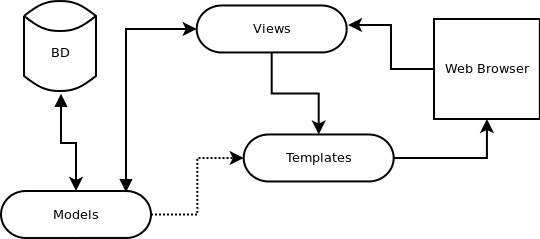
\includegraphics[width=0.7\textwidth]{fig/DjangoMVT.png}
	\caption[Diagrama patrón MVT]{Diagrama patrón MVT \footnotemark}
	\label{fig:ej1}
\end{figure}
\footnotetext{https://docs.hektorprofe.net/django/web-personal/patron-mvt-modelo-vista-template/}

Para poder trabajar con bases de datos relacionales tales como, Oracle, MySQL y PostgreSQL, Django usa un Mapeador Relacional de Objetos (ORM) que permite interactuar con ellas mediante SQL.\newline
\newline
Django es uno de los frameworks más reputados en Python, teniendo en cuanta su naturaleza gratuita y de código abierto. Siendo usado tanto por la comunidad como por empresas tales como Instagram, Mozilla y Facebook. Aunque no por ello significa que no disponga de poca competencia, siendo TurboGears, web2py, Bottle y Flask de las más notables.
\newline
\newline
El que sea un framework full-stack no va a aportar la flexibilidad, libertad y ligereza que da el uso de un microframework, sobre todo a la hora de agregar únicamente aquellas herramientas que considere necesarias, pero si que atenuará la carga de trabajo que puede suponer un microframework si no se dispone de la experiencia necesaria para usarlo.
\newline
\newline
Otra característica por la que decantarse por Django, aunque no sea única de él, es su compatibilidad con bases de datos relacionales de forma nativa, cosa que facilitará el uso de estas en el proyecto.\newline
\newline
A su vez, con el fin de obtener los datos, se necesita de una herramienta centrada en el scrapeo de datos.

\section{Herramienta para Web Scraping}
Web scraping, también conocido como web extraction o web harvesting, es una técnica de extracción de datos desestructurados de la World Wide web (WWW) y guardarlos de forma estructurada en una base de datos o en un sistema de ficheros en formato XML, JSON o CSV para su posterior recuperación o análisis. Generalmente, los datos web son adquiridos mediante el uso de Hyper-text Transfer Protocol (HTTP) o a través de un navegador web, ya sea de forma manual o automática mediante web crawlers, herramientas diseñadas con este propósito, siendo capaces de convertir páginas web enteras en información bien estructurada \cite{zhao2017web} \cite{krotov2018legality}.
\newline
\newline
Debido a la gran cantidad de datos que son generados constantemente en la WWW, web scraping es considerado una forma eficiente y poderosa de amasar big data. Pudiendose usar en una gran variedad de entornos, como la recolección de comentarios en redes sociales, listado de la propiedad inmobiliaria o en este caso el monitoreo y comparación de los niveles de los ríos y datos pluviométricos.

\subsection{Procedimiento básico en Web Scraping}
El proceso de recolección de datos de Internet se puede dividir en tres procesos secuenciales, el estudio de la pagina sobre la que trabajar, adquirir los recursos web y, luego, organizar la información deseada. Como se ve en la figura \ref{fig:ej2}.
\newline
\newline
El primer paso consiste en mirar la estructuración de la web para seleccionar aquellos datos que queramos extraer, comprobando los recursos HTML, CSS y viendo si hace uso de JavaScript. Para realizar el segundo paso de adquisición de los recursos, el proceso empieza con los programas de web scraping enviando un request, ya sea mediante GET o POST, a la página web deseada. Una vez el request sea recibido y procesado por la web, esta enviará los recursos solicitados al programa. Después, pasaríamos al tercer paso, en el que analizaríamos los recursos obtenidos y los filtraríamos de tal forma que nos quedásemos únicamente con la información que nos sea necesaria. Finalmente almacenaríamos la información obtenida para su posterior análisis.
\newline
\begin{figure} [h!]
	\centering
	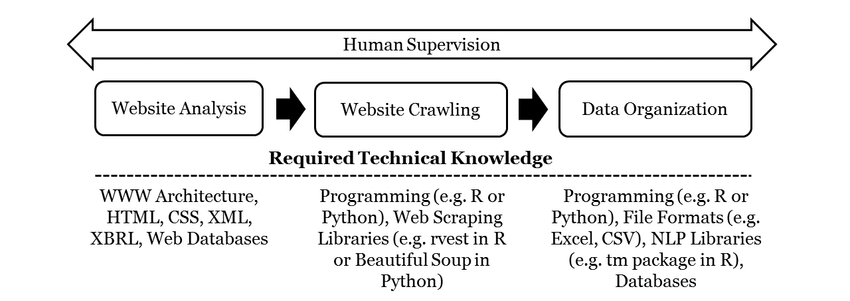
\includegraphics[width=0.7\textwidth]{fig/Web-Scraping-Adapted-from-Krotov-and-Tennyson-2018.png}
	\caption[Web Scraping (Krotov y Tennyson 2018)]{Web Scraping \footnotemark}
	\label{fig:ej2}
\end{figure}
\footnotetext{\url{https://www.researchgate.net/figure/Web-Scraping-Adapted-from-Krotov-and-Tennyson-2018_fig1_324907302}}

\subsection{Scrapy Framework}
Scrapy es un framework asíncrono para web crawling y web scraping gratuito y de código abierto. Por defecto proporciona todas las herramientas necesarias para realizar la tarea de extracción, procesado y estructurado de los datos adquiridos, ademas de dar la opción de extender funcionalidades en caso necesario, haciéndolo extremadamente versátil \cite{yang2019design}.
\newline
\newline
Pensado para navegar entre webs y extraer información de forma estructurada de ellas, Scrapy se usa para múltiples ámbitos, por ejemplo, el minado de datos o la monitorización y análisis de datos.\newline
\newline
A la hora de buscar herramientas para web scraping en Python, fueron tres la alternativas principales encontradas, BeautifulSoup, Selenium y Scrapy.
\newline
\newline
La primera es una librería de parseo de HTML y XML, que, aunque podría haber servido para cumplir el propósito del proyecto inicialmente, a la larga su sencillez hubiera sido más un problema que una ayuda.
\newline
\newline
La segunda por el contrario, no es una herramienta de web scraping como tal y, se centra en la automatización de la navegación web como entorno de pruebas. Debido a esto, no es una herramienta que haya usado para el web scraping, pero si que ha sido usada junto con Scrapy para navegar entre webs y sacar los datos de estas. Proporcionando la posibilidad de hacer uso de JavaScript sobre las páginas, pues Scrapy no dispone de renderizado JavaScript de forma nativa.
\newline
\newline
Scrapy fue elegido gracias a la flexibilidad y versatilidad que proporciona a la hora de trabajar, pudiendo crear proyectos sencillos en cuestión de minutos con las herramientas base proporcionadas o investigar como trabajar con estas herramientas y crear proyectos complejos que satisfagan tus necesidades de la manera que desees. Esto implica que la curva de aprendizaje de Scrapy sea mayor que la que puede tener BeautifulSoup, sobre todo al inicio, llegando a parecer abrumador. A su vez, la naturaleza de Scrapy le hace tener el mejor rendimiento de entre las tres \cite{glez2014web}.
\newline
\newline
Finalmente, cabe mencionar que Scrapy no dispone de rotación de IP, ni geolocalización como pueden tener las alternativas de pago, cosa que no es un impedimento para llevar a cabo el proyecto.\newline
\newline
Para satisfacer el segundo servicio necesario se requerirá de una base de datos.

\section{Base de Datos}
Debido a la naturaleza de los JSON obtenidos, se pueden trasladar fácilmente a tablas relacionales, por lo que se hará uso de una base de datos relacional.

\subsection{PostGreSQL}
PostGreSQL, es un sistema de gestión de bases de datos relacional de código abierto. PostgreSQL destaca por su sistema de gestión de bases de datos, su soporte para consultas complejas, transacciones ACID, integridad referencial y escalabilidad.\newline
\newline
Además, ofrece una amplia gama de tipos de datos, incluyendo geoespaciales y JSONB, almacenando JSONs de forma binaria (de ahí la B) para su fácil acceso.\newline
\newline
La comunidad activa detrás de PostgreSQL contribuye continuamente con mejoras y extensiones, lo que lo convierte en una solución versátil y confiable. Lo que la hace popular tanto para aplicaciones empresariales como para proyectos web.\newline
\newline
Entre las bases de datos con soporte oficial en Django se encuentran, PostgreSQL, MariaDB, MySQL, Oracle y SQLite. A excepción de Oracle, la única base de datos comercial, el resto son de código abierto, aunque puedan disponer de versiones de pago.\newline
\newline
A nivel de funcionalidades, todas ofrecen implementadas de una forma u otra una misma gama de estas. Es por eso que, la elección se hizo en base a la flexibilidad y robustez de estas. Lo que hace a PostGreSQL una opción interesante en proyectos que lleguen a requerir de datos geoespaciales y JSON.

\subsection{Arquitectura Preliminar}
Tras la selección de las herramientas a usar, la arquitectura queda de las manera mostrada en la figura \ref{fig:ej9}. Como herramienta de scraping, el framework Scrapy; como base de datos PostGreSQL y, como servicio API el framework Django.

\begin{figure} [H]
	\centering
	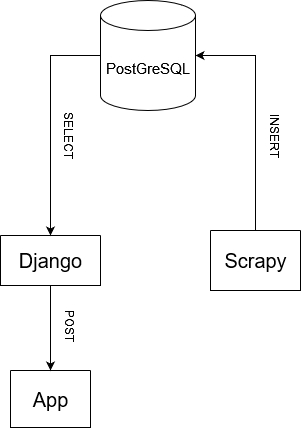
\includegraphics[width=0.3\textwidth]{fig/estructura_descartada.png}
	\caption[Idea original de la estructura de datos planteada]{Estructura descartada}
	\label{fig:ej9}
\end{figure}

El hecho de seleccionar estos Framework, impone la necesidad de usar como lenguaje de programación Python.\newline
\newline
Siendo su primera aparición en el año 1991 por manos de Guido van Rossum, Python es un lenguaje de programación de alto nivel interpretado que prima la legibilidad del código, siendo este a veces nominado como "seudocódigo ejecutable" \cite{dierbach2014python}. Python a su vez es un lenguaje multiplataforma, fuertemente tipado, dinámico y multiparadigma, pues soporta programación orientada a objetos, imperativa y funcional \cite{PyDoc} \cite{borges2014python}.

\chapter[Datos]{Datos}
\label{Chap2}

Para este proyecto se dispone de los siguientes datos:
\begin{itemize}
	\item Nivel (m)
	\item Caudal ($m^3/s$)
	\item Precipitación (mm)
	\item Temperatura (ºC)
	\item Humedad (\%)
	\item Radiación ($W/m^2$)
\end{itemize}
A su vez, se dispone de la fecha y hora en la que se hicieron la lectura de los datos, junto con los códigos y coordenadas de las estaciones sobre las cuales se obtienen los datos.

\section{Aemet}
Como se ve en la imagen \ref{fig:ej3}, dentro de la web podemos encontrar de forma accesible múltiples datos relacionados con la meteorología tomados cada hora, de los cuales seleccionaremos únicamente temperatura, precipitación y humedad, puesto que los datos relacionados con el viento no son tan relevantes para este proyecto. A su vez, no todas las estaciones muestran estos datos, ocurriendo lo mismo con los de presión atmosférica.

\begin{figure} [H]
	\centering
	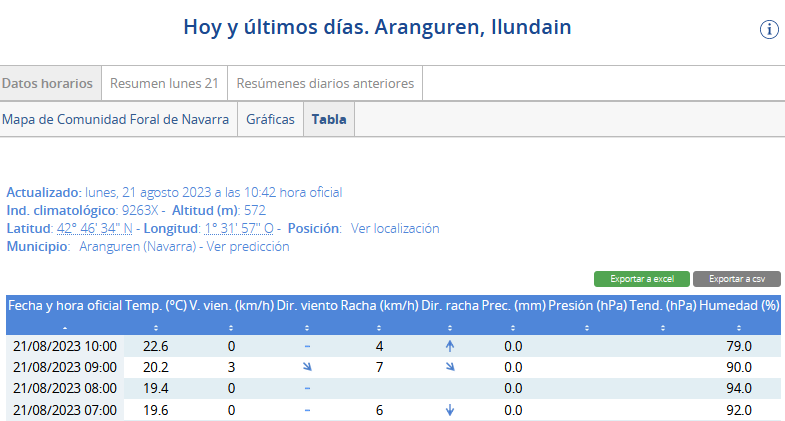
\includegraphics[width=0.7\textwidth]{fig/AemetData.png}
	\caption[Página Aemet de la estación en Aranguren (Navarra)]{Página Datos Aemet}
	\label{fig:ej3}
\end{figure}

Los datos en HTML vienen datos dentro de un elemento tabla, imagen \ref{fig:ej20}, lo que facilita su adquisición, pues permite tomar todas las filas (elementos tr) pertenecientes al elemento tbody de esta. Una vez obtenidas las filas, la forma de lograr los datos deseados seria eligir dentro de cada elemento tr los elementos td deseados, puesto que HTML empieza a contar elementos desde el uno (en vez de cero como suele ser común en lenguajes de programación), los td a obtener serian: uno, fecha y hora; dos, temperatura; siete, precipitación; diez, humedad.

\begin{figure} [H]
	\centering
	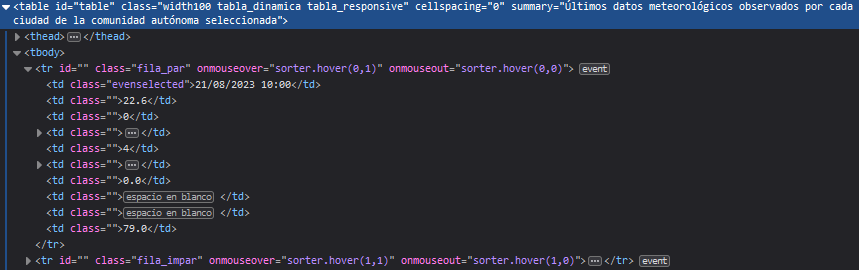
\includegraphics[width=0.7\textwidth]{fig/AemetDataHTML.png}
	\caption[HTML de la tabla de datos de Aemet de la estación en Aranguren (Navarra)]{HTML Tabla Datos Aemet}
	\label{fig:ej20}
\end{figure}

Las coordenadas, dentro de un span, imagen \ref{fig:ej21}, están incluidas en elementos abbr con sus respectivas clases "latitude" y "longitude", haciendo posible su obtención fácilmente mediante los elementos abbr.

\begin{figure} [H]
	\centering
	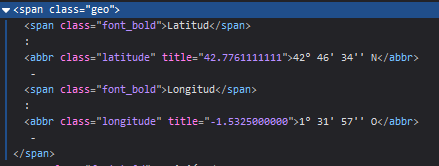
\includegraphics[width=0.7\textwidth]{fig/AemetCoordHTML.png}
	\caption[HTML de las coordenadas de Aemet de la estación en Aranguren (Navarra)]{HTML de las coordenadas en Aemet}
	\label{fig:ej21}
\end{figure}

\section{El Agua en Navarra}
En esta página encontraremos los datos tanto del nivel de los ríos como de su caudal en los últimos 15 días en periodos de 10 minutos, siendo una de las fuentes principales de datos.
\newline
\newline
La sección de aforos en la página, imagen \ref{fig:ej4}, muestra el mapa de Navarra junto a varias estaciones. Aunque no todas las disponibles en la web, conformando unicamente el grupo de estaciones principales.\newline
\newline
Con el fin de acceder a todas las estaciones disponibles, debemos centrarnos en el mapa de la esquina inferior derecha. Estructurada en 6 regiones, Norte, Arga, Ega, Ebro alto, Ebro bajo y Aragón, por medio de este mapa accedemos a cada región, mostrando el mapa de la región, dando acceso a todas las estaciones en la zona.

\begin{figure} [H]
	\centering
	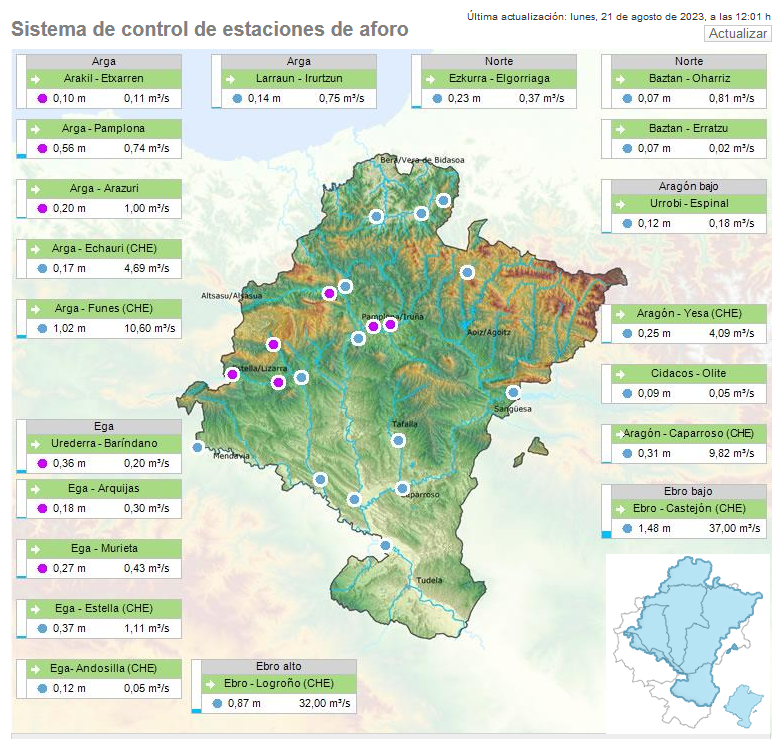
\includegraphics[width=0.7\textwidth]{fig/AguaEnNavarraCode.png}
	\caption[Página principal de aforos de El Agua en Navarra]{Página El Agua en Navarra}
	\label{fig:ej4}
\end{figure}

El HTML del mapa se estructura de la siguiente manera, imagen \ref{fig:ej22}, mostrando un par de elementos area por estación, uno con shape "rect", representando las tarjetas que rodean el mapa y otro con shape "circle", siendo los puntos en el mapa. Pulsar sobre cualquiera de ellos es equivalente, aunque posteriormente hagamos uso de los elementos "rect" dentro del código.

\begin{figure} [H]
	\centering
	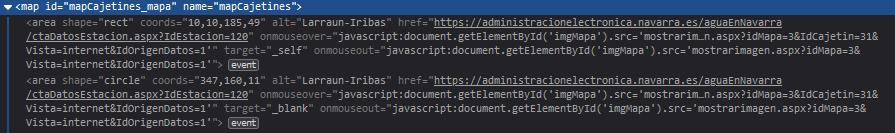
\includegraphics[width=0.7\textwidth]{fig/AguaEnNavarraCodeHTML.png}
	\caption[HTML mapa estaciones de El Agua en Navarra]{HTML mapa estaciones El Agua en Navarra}
	\label{fig:ej22}
\end{figure}

Las paginas de cada estación se muestran como en la imagen \ref{fig:ej23}.

\begin{figure} [H]
	\centering
	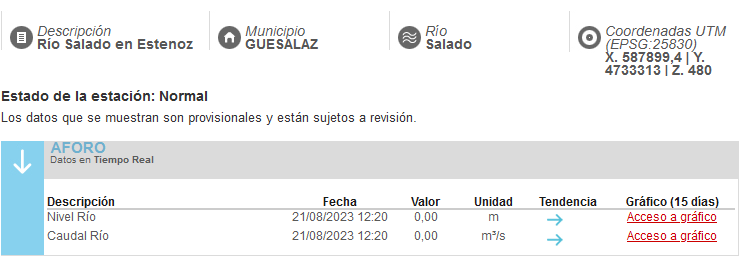
\includegraphics[width=0.7\textwidth]{fig/AguaEnNavarraEstacion.png}
	\caption[Página estación de El Agua en Navarra]{Página estación El Agua en Navarra}
	\label{fig:ej23}
\end{figure}

De ella obtenemos los próximos datos, descripción, municipio, río y coordenadas. Ademas de darnos acceso a los datos de nivel y caudal del río. Mostrados dentro de el div con id "blog\_icons", imagen \ref{fig:ej24}. Una vez dentro del div todos los datos siguen la misma estructuración, //div/span/span, permitiendo la adquisición de todos los elementos a la vez.

\begin{figure} [H]
	\centering
	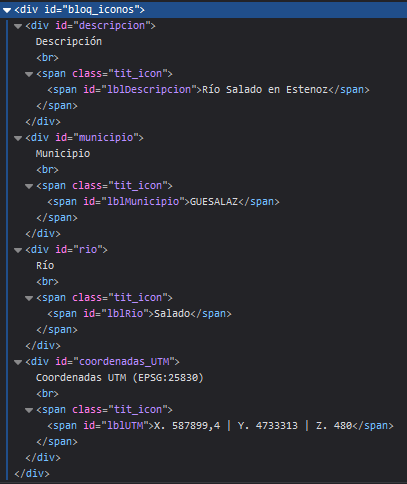
\includegraphics[width=0.7\textwidth]{fig/AguaEnNavarraEstacionHTML.png}
	\caption[HTML estación de El Agua en Navarra]{HTML estación El Agua en Navarra}
	\label{fig:ej24}
\end{figure}

Una vez se accede a los datos de la estación, se mostrara una gráfica como la de la imagen \ref{fig:ej25}. A su vez, mediante el botón "Datos Numéricos", tendremos la posibilidad de observar los datos en forma numérica. Pero no sin antes haber visitado la versión gráfica. Pues da el error de la imagen \ref{fig:ej5}.

\begin{figure} [H]
	\centering
	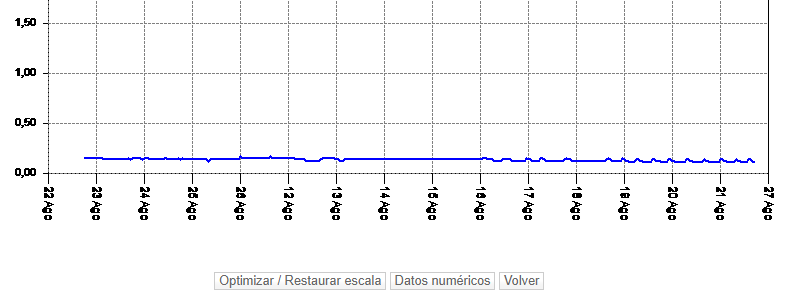
\includegraphics[width=0.7\textwidth]{fig/AguaEnNavarraGrafica.png}
	\caption[Gráfica de datos en estación de El Agua en Navarra]{Gráfica datos estación El Agua en Navarra}
	\label{fig:ej25}
\end{figure}

\begin{figure} [H]
	\centering
	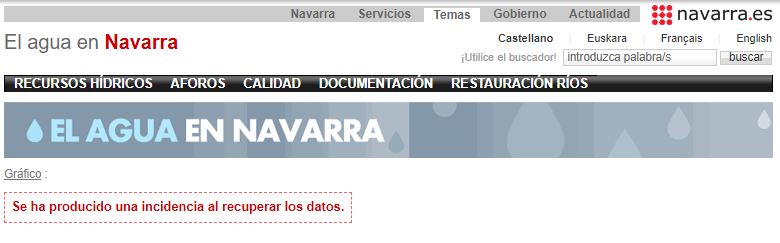
\includegraphics[width=0.7\textwidth]{fig/ErrorAguaEnNavarra.png}
	\caption[Error al cargar directamente la página de datos numéricos en El Agua en Navarra]{Error datos numéricos en El Agua en Navarra}
	\label{fig:ej5}
\end{figure}

Los datos numéricos están presentados en formato tabla como se aprecia en la imagen \ref{fig:sub3}. Por el contrario, tras observar el HTML, realmente es un elemento div, que engloba los conjuntos de elementos span que representan las lineas, separados por elementos br, imagen \ref{fig:sub4}. El formato en el que se presentan los datos, no hace más que representar una mayor complejidad para, posteriormente, trabajar y adquirir los datos. 

\begin{figure} [H]
	\centering
	\begin{subfigure}{.5\textwidth}
		\centering
		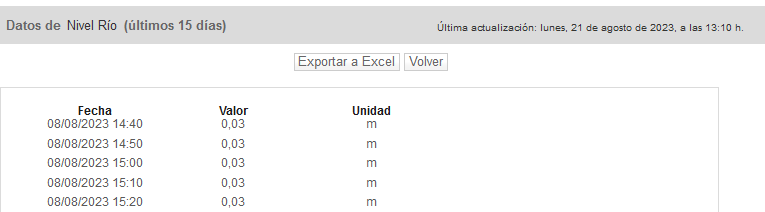
\includegraphics[width=.9\linewidth]{fig/AguaEnNavarraData.png}
		\caption{Formato presentación de los datos}
		\label{fig:sub3}
	\end{subfigure}%
	\begin{subfigure}{.5\textwidth}
		\centering
		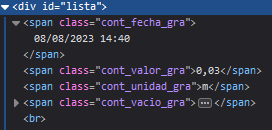
\includegraphics[width=.7\linewidth]{fig/AguaEnNavarraDataHTML.png}
		\caption{HTML de los datos}
		\label{fig:sub4}
	\end{subfigure}
	\caption{Datos numéricos de estaciones en Agua en Navarra}
	\label{fig:ej26}
\end{figure}

\section{MeteoNavarra}
En la página de meteorología y climatología de Navarra encontramos una gran sección de estaciones de las cuales poder obtener datos. Imagen \ref{fig:ej27}.

\begin{figure} [H]
	\centering
	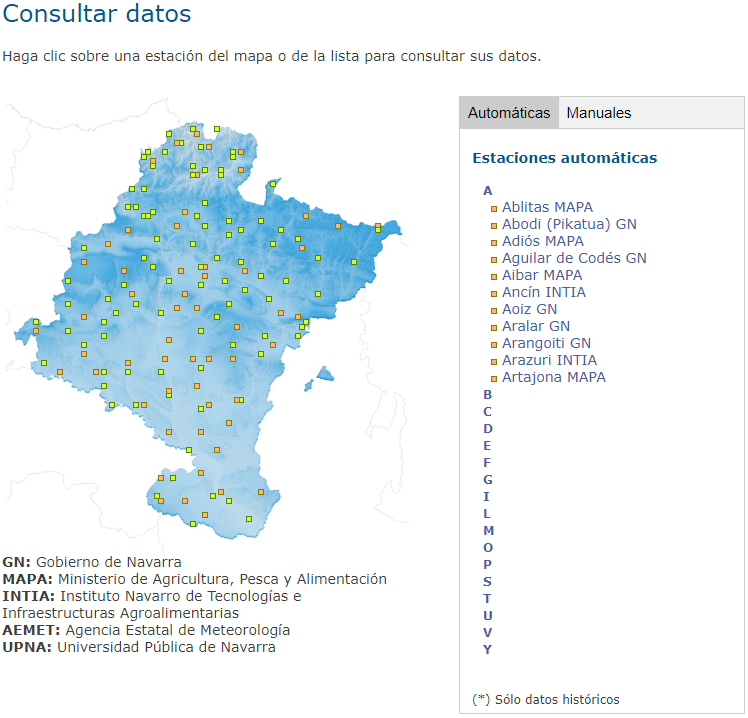
\includegraphics[width=0.7\textwidth]{fig/MeteoNavarraCode.png}
	\caption[Página estaciones MeteoNavarra]{Página estaciones MeteoNavarra}
	\label{fig:ej27}
\end{figure}

De entre los dos tipos e estaciones disponibles, automática y manual, únicamente se va a trabajar con los datos de las estaciones automáticas. El motivo de esto es que las manuales solo proveen datos diarios de, la temperatura máxima, mínima y de la precipitación acumulada. Esto hace que no se disponga de ningún dato hasta que finalice el día, cosa que no es viable si lo que se propone es predecir cambios radicales en un periodo de tiempo reducido.
\newline
\newline
Debido a la estructuración HTML usada para mostrar las estaciones, imagen \ref{fig:sub5}, se puede ver que aun usar el elemento table, este solo dispone de una única fila y columna, haciendo de la columna un elemento div sobre el que insertar los datos, imagen \ref{fig:sub6}. Como es el caso de la web de Agua en Navarra.

\begin{figure} [H]
	\centering
	\begin{subfigure}{.5\textwidth}
		\centering
		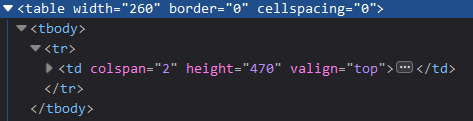
\includegraphics[width=.7\linewidth]{fig/MeteoNavarraCodeHTMLTable.png}
		\caption{Tabla}
		\label{fig:sub5}
	\end{subfigure}%
	\begin{subfigure}{.5\textwidth}
		\centering
		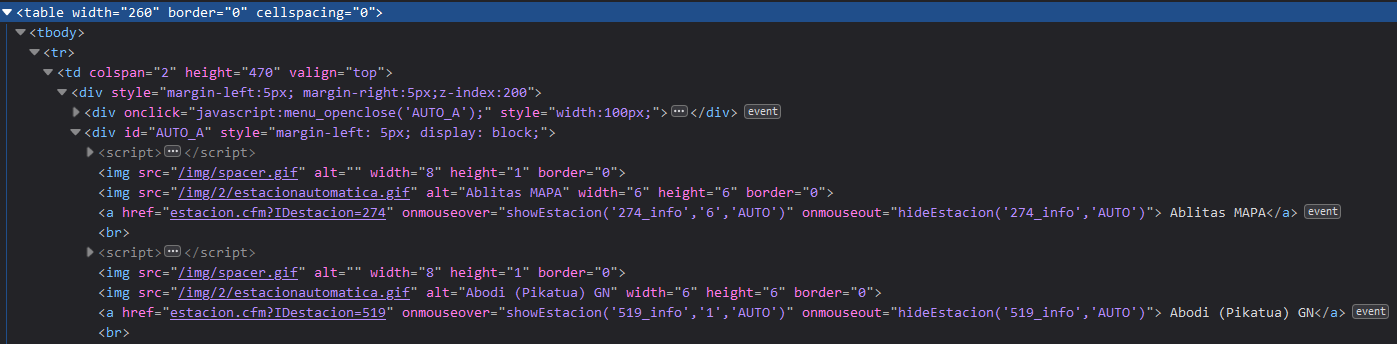
\includegraphics[width=.7\linewidth]{fig/MeteoNavarraCodeHTML.png}
		\caption{Filas}
		\label{fig:sub6}
	\end{subfigure}
	\caption{HTML tabla estaciones MeteoNavarra}
	\label{fig:ej28}
\end{figure}

Las estaciones automáticas proporcionan tanto datos en periodos de diez minutos como datos diarios. Tras usar el mismo razonamiento que con las estaciones manuales, no tomamos los datos diarios y, entre los actualizados cada diez minutos, se toman la temperatura, humedad relativa, radiación global y precipitación. El resto se omitirán. Imagen \ref{fig:ej6}.

\begin{figure} [H]
	\centering
	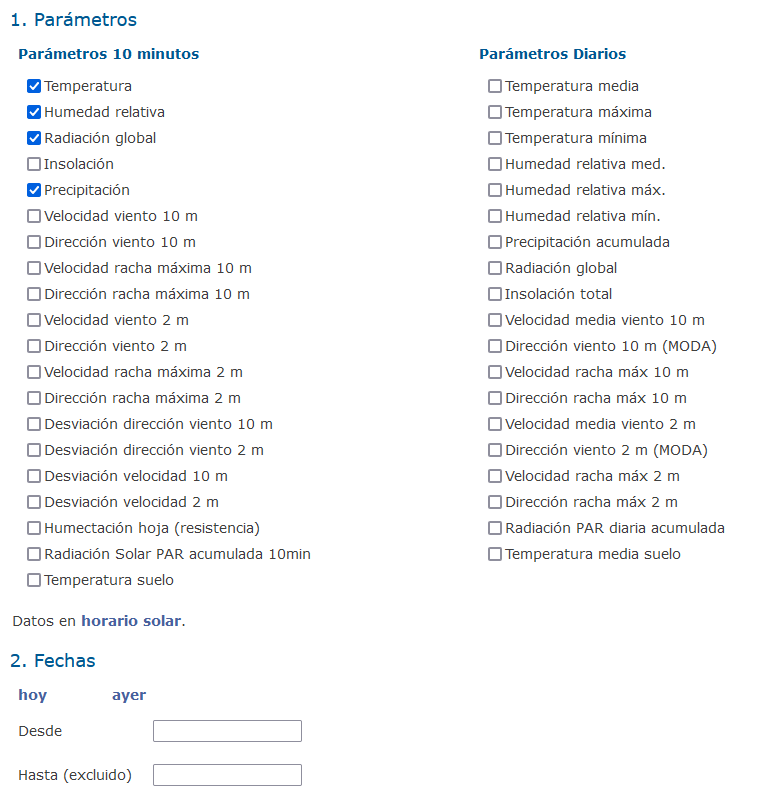
\includegraphics[width=0.7\textwidth]{fig/DatosMeteoNavarra.png}
	\caption[Apartado selección de datos MeteoNavarra]{Datos MeteoNavarra}
	\label{fig:ej6}
\end{figure}

Los datos se muestran en formato tabla, tanto visualmente, en la imagen \ref{fig:sub7} como a nivel de HTML, imagen \ref{fig:sub8}, cosa que facilita su obtención.

\begin{figure} [H]
	\centering
	\begin{subfigure}{.5\textwidth}
		\centering
		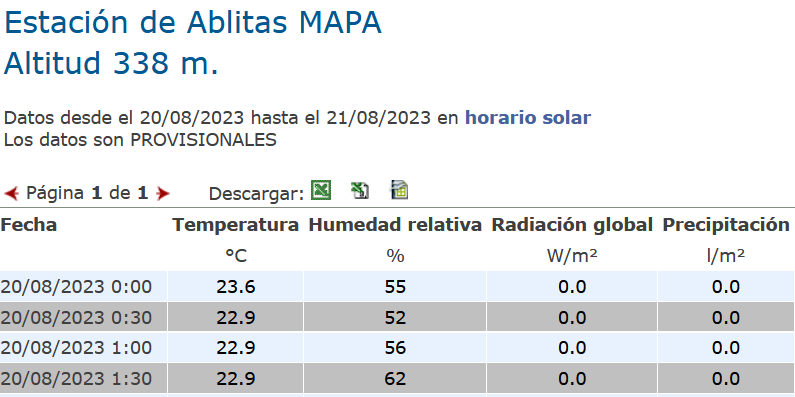
\includegraphics[width=.7\linewidth]{fig/MeteoNavarraData.png}
		\caption{Tabla datos}
		\label{fig:sub7}
	\end{subfigure}%
	\begin{subfigure}{.5\textwidth}
		\centering
		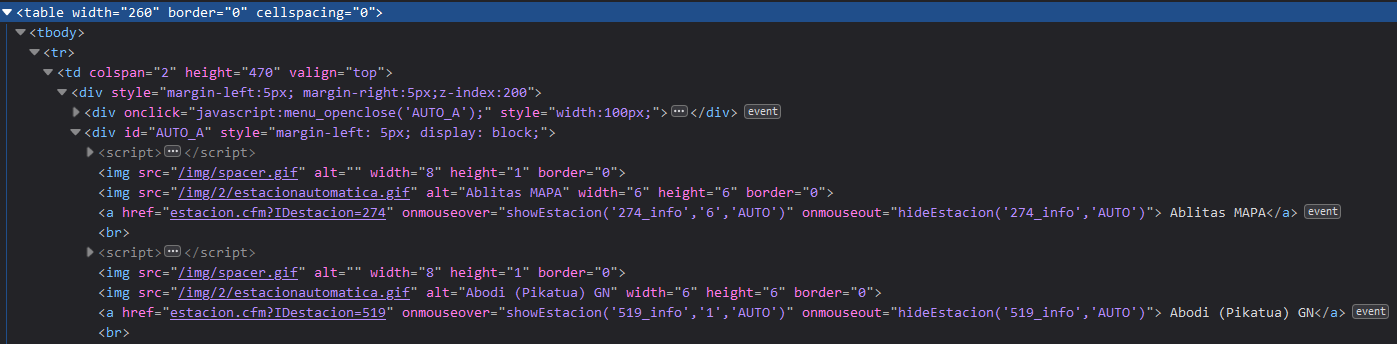
\includegraphics[width=.7\linewidth]{fig/MeteoNavarraCodeHTML.png}
		\caption{HTML de la tabla de datos}
		\label{fig:sub8}
	\end{subfigure}
	\caption{Página de datos de MeteoNavarra}
	\label{fig:ej29}
\end{figure}

\section{CHCantábrico}
En la sección de nivel del río de la pagina de CHCantábrico, se encuentra la tabla con las estaciones, imagen \ref{fig:sub9}. Una peculiaridad de esta, es que aun seguir una estructuración típica de tabla mediante el uso de table, dispone de una tabla adicional en cada una de las filas. Imagen \ref{fig:sub10}.

\begin{figure} [H]
	\centering
	\begin{subfigure}{.5\textwidth}
		\centering
		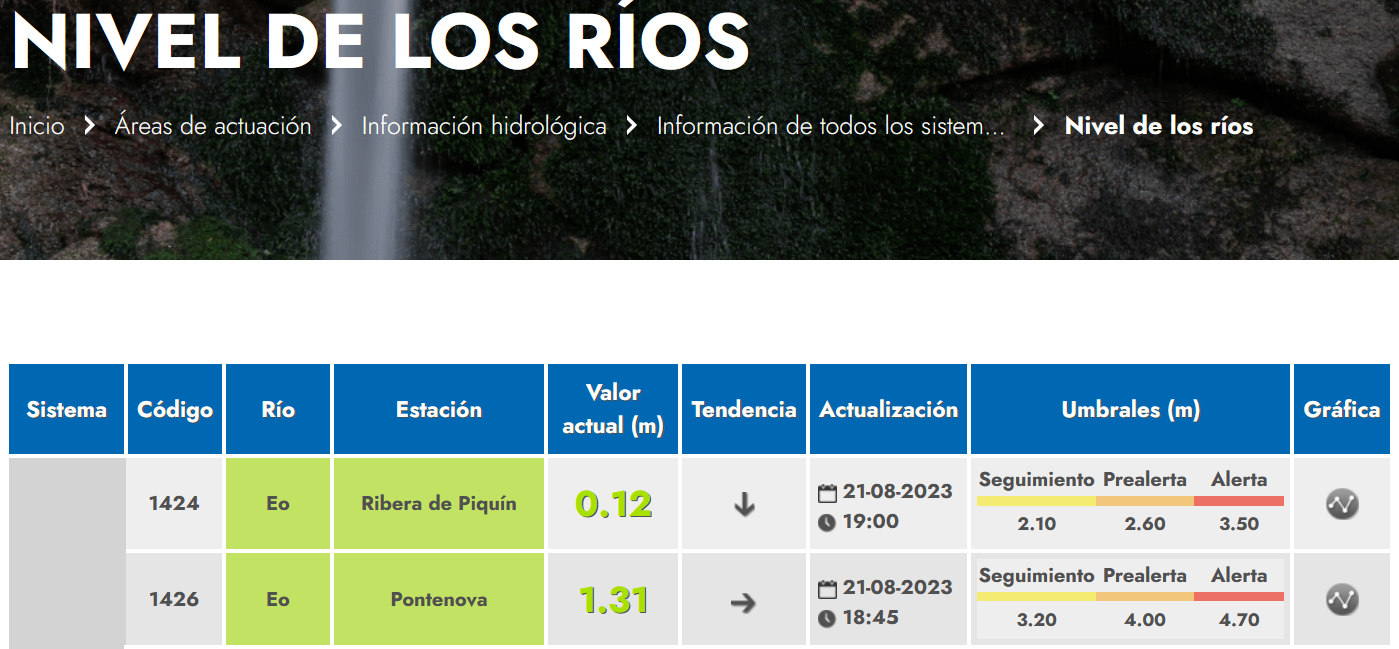
\includegraphics[width=.7\linewidth]{fig/CHCantabricoCode.png}
		\caption{Tabla estaciones}
		\label{fig:sub9}
	\end{subfigure}%
	\begin{subfigure}{.5\textwidth}
		\centering
		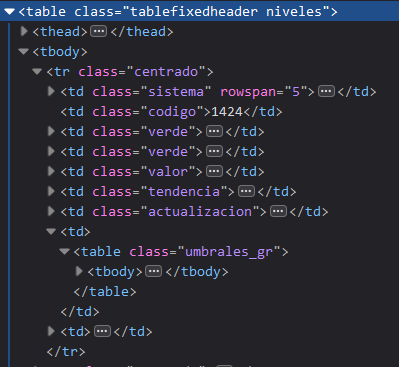
\includegraphics[width=.7\linewidth]{fig/CHCantabricoCodeHTML.png}
		\caption{HTML de la tabla de estaciones}
		\label{fig:sub10}
	\end{subfigure}
	\caption{Página Nivel de los ríos CHCantábrico}
	\label{fig:ej30}
\end{figure}

A diferencia del resto de las páginas visitadas, CHCantábrico no muestra los datos sobre la web, por el contrario, implementa un botón con el que descargarlos directamente en formato CSV. Más adelante en el documento se discutirá la repercusión de ello.\newline
\newline
Los datos que si se pueden obtener, son aquellos presentes en la tabla secundaria de las fila, los datos de pre-alerta, alerta y seguimiento para cada una de las estaciones, siendo datos valiosos a la hora de intentar anticipar inundaciones.\newline
\newline
Las coordenadas a su vez, tampoco vienen dados sobre la web, por lo que hace falta visitar la web del Centro de Estudios Hidrológicos (\url{https://ceh.cedex.es/}) para obtenerlas.
\chapter[Evaluación]{Evaluación}
\label{Chap4}

\section{Estructuras Planteadas}

Scrapy -INSERT-> PostGreSQL <-SELECT- Django -POST-> App\newline
Problema: aunque sea la estructura más simple y fácil de implementar, pues scrapy mismo puede insertar los datos scrapeados de las web de forma directa en PostGreSQL, Djando hace uso de un sistema de gestión de versiones de los cambios realizados en la BBDD con el fin de reducir la carga de peticiones a la BBDD, esto se aplica desde el lado de Django, lo que supondría un problema a la hora de insertar datos directamente de Scrapy a PostGreSQL, pues los nuevos datos podrían no llegar a ser detectados por Django, generando la situación de que una vez se vayan a pedir los nuevos datos Django no devuelva nada pues desde su punto de vista los datos que ya dispongo son la versión mas reciente, luego no es necesario realizar llamada alguna a la BBDD.
\newline
\newline
Scrapy -POST JSON-> Django -INSERT-> PostGreSQL <-SELECT- Django -POST-> App\newline
Solución: Pasa solventar el problema hemos incluido un paso intermedio en el que inicialmente almacenamos los datos obtenidos de las distintas webs en formato JSON, para posteriormente enviárselos a Django, el cual se encargara de subir los datos a la BBDD, mientras, el resto de la arquitectura seria idéntico a la versión original.

\section{Trabalho 2}
Flujo de datos:\newline

1.- Pedir datos (JSON1)\newline
2.- Formatear datos en un nuevo JSON (JSON1 -> JSON2)\newline
3.- Mandar datos a la BBDD (JSON2)\newline
4.- Marcar JSON como old (JSON2 -> JSON3)\newline
5.- Borrar JSON original (JSON1)\newline

While(true)\newline
	1.- Pedir datos (JSON1)\newline
	2.- Formatear datos en un nuevo JSON (JSON1 -> JSON2)\newline
	6.- Crear JSON con las nuevas fechas (JSON2 != JSON3 y fecha de hoy -> JSON4)\newline
	7.- Mandar datos a la BBDD (JSON4)\newline
	4.- Marcar JSON como old (JSON2 -> JSON3)\newline
	5.- Borrar JSON original (JSON1)\newline
	8.- Borrar JSON viejo (JSON3)\newline
	9.- Borrar JSON diferencias (JSON4)\newline
\newline
\newline
Puesto que los datos obtenidos no son los mismos para cada web, antes de ser enviados a Django deben ser parseados para compartir una estructura heterogénea, una vez obtenido el JSON parseado, en caso de ser la primera iteración se mandaran directamente los datos a la BBDD, de no ser la primera iteración, se tomaran unicamente los nuevos datos obtenidos como datos a enviar, una vez enviados los datos el JSON parseado sera marcado como old (viejo) para ser el punto de comparación respecto a los datos mas recientes que obtendremos de las webs.

\subsection{Trabalho 2.1}
Datos obtenidos:\newline
Aemet:\newline
temperatura, humedad, precipitación
\newline
meteoNavarra:\newline
temperatura, humedad, precipitación, radiación
\newline
aguaEnNavarra:\newline
nivel, caudal
\newline
chcantabrico:\newline
nivel, precipitación, seguimiento, alerta, pre-alerta

En todas las webs se proporciona las coordenadas junto con la fecha y hora en la que se ha hecho la medida

\subsection{Trabalho 2.2}
No todas las webs presentan sus datos de la misma manera, es por eso que nos encontramos con que los datos que hemos obtenido pueden llegar a estar repartidos en distintas páginas, haciendo necesario el uso de múltiples spiders, resultando en multiples JSON.
Es por eso que para cada web se ha creado una función para parsear (formatear) los datos obtenidos, de esta manera disponemos de una estructura única para los datos recibidos, haciendo su uso posterior más fácil, ya sea a la hora de tratarlos posteriormente como para almacenarlos en la base de datos

Esquema obtenido:
\newline
\newline
\newline
[
\{
	"coordenadas": "X. 598270,3 | Y. 4659333 | Z. 37928",
	"estacion": "64",
	"datos": [
	\{
		"fecha y hora": "01/06/2023 11:20:00",
		"temperatura (ºC)": null,
		"humedad (\%)": null,
		"precipitacion (mm)": null,
		"nivel (m)": "0,05",
		"caudal ($m^3/s$)": null,
		"radiacion ($W/m^2$)": null
	\}
	]
\}
]

\subsection{Trabalho 2.3}
Una vez formateados los datos con el fin de reducir la carga a la base de datos, estos son filtrados mediante la comparación con los ficheros anteriormente marcados como old, de esta forma nos aseguramos de mandar a la base de datos unicamente las instancias nuevas de los datos recogidos, pues no disponemos de ninguna forma para filtrar los datos a la hora de obtenerlos. Estos datos serán guardados en un tercer JSON.

\section{Arquitectura}
Para poder realizar el trabajo se ha diseñado la siguiente arquitectura.\ref{fig:ej7}
\begin{figure} [h]
	\centering
	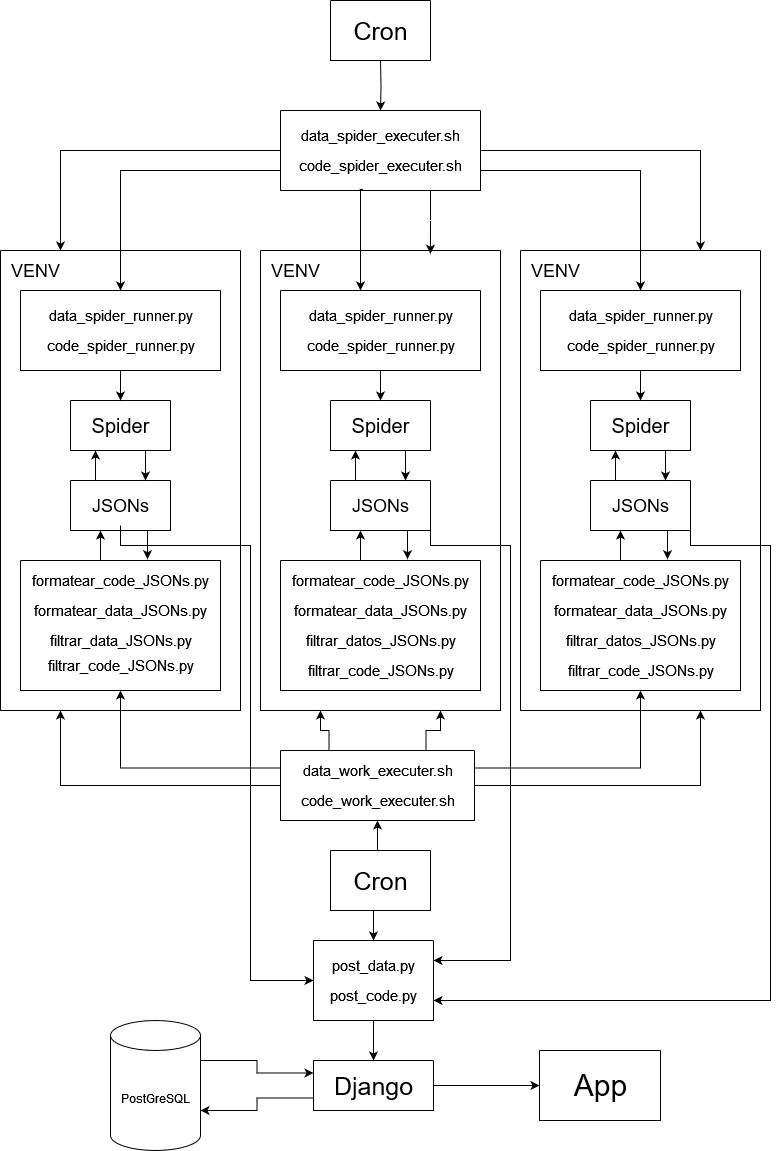
\includegraphics[width=0.7\textwidth]{fig/arquitectura.png}
	\caption[Arquitectura de obtención y tratamiento de datos]{Arquitectura de obtención y tratamiento de datos}
	\label{fig:ej7}
\end{figure}

\subsection{Elementos presentes}

\subsubsection{Entornos virtuales}
Con el fin de que la plataforma sea lo mas fácilmente ampliable se ha decidido que cada Spider disponga de su propio entorno virtual, esto permite añadir dependencias de tal forma que no afecten a el resto de los Scripts presentes, ayudando en la encapsulación de dependencias.
El mayor inconveniente de una plataforma así es la redundancia de código, al ser múltiples entornos independientes es necesario que mucho código sea repetido en cada uno de ellos, cosa que si fuera un único entorno en el que se ejecutara todo, con una clase sobre la que heredar y o una interfaz, seria mucho el código que nos ahorraríamos.
Actualmente la plataforma dispone de cuatro entornos virtuales para cada Spider y un entorno virtual sobre el que ejecutar el servidor de Django.

\subsubsection{Spiders}
Cada Spider representa una web, de tal forma que cada una de ellas obtiene los datos de la web sobre la que se ha diseñado exclusivamente, para poder realizar esta tarea por cada web han sido necesarias varias Spider, aunque de forma simplificada se pueden agrupar por, aquellas que obtienen las estaciones junto con sus códigos y, las de obtención de datos.
De esta forma dividimos las tareas dándonos la posibilidad de ejecutar aquella que mejor nos venga en cada momento.

\subsubsection{Runners}
Runner es la forma en la que han sido nombrados los Scripts cuya función es posibilitar la ejecución en nuestro caso asíncrona de una o múltiples Spiders mediante un único comando.
Es un Script simple en el que una vez dispones de la estructura básica en caso de necesitar añadir o eliminar una Spider solo tienes que agregar o eliminar la Spider en cuestión y ya estaría listo.
A su vez, al añadir un intermediario el comando de ejecución pasa de ser, scrapy crawl nombreSpider por cada Spider que se desea ejecutar, a, python nombreRunner.py facilitando la automatización de ejecución de las Spider.

\subsubsection{Executers}
Aumentado un poco mas la abstracción nos encontramos con los Executers, Scripts en Bash encargados de activar el entorno virtual de la Spider deseada y acto seguido ejecutar su respectivo Runner.
Estos existen (en mayor medida que los Runners) con el fin de ayudar con el mantenimiento de la arquitectura, creando un nuevo intermediario en la cadena de ejecución.
Están diseñados de tal forma que funcionen pasandoles un único argumento representando la web de la que quieres obtener los datos, haciendo que la agregación de nuevas Spiders junto con sus entornos sea tan sencillo como respetar las rutas y nombres predefinidos.

\subsubsection{JSONs}
Este apartado es un conjunto de directorios en los que se van almacenando los JSON obtenidos tras los distintos procesos a los que son sometidos.
Los directorios en cuestión, siguiendo orden de creación para los JSON de datos son los siguientes:
\begin{enumerate}
	\item RawData
	\item ParsedData
	\item RefinedData
	\item OldData
\end{enumerate}
Y los de códigos (estación):
\begin{enumerate}
	\item RawCode
	\item ParsedCode
	\item RefinedCode (TODO)
	\item OldCode (TODO)
\end{enumerate}
El primer nivel es aquel que se obtiene de la llamada con la Spider a la web, devolviendo todos los datos de esta.\newline
El segundo, es obtenido tras ejecutar ya sea formatear\_data\_JSONs.py en caso de querer parsear los datos o formatear\_code\_JSONs.py para los códigos.\newline
El tercero se obtiene tras eliminar la duplicidad de datos en comparación con los ya almacenados en la base de datos mediante la ejecución de filtrar\_data\_JSONs.py.\newline
Finalmente el cuarto es el subproducto obtenido tras la comparación, tomando el fichero original ya formateado y cambiándole de directorio y el nombre de tal forma que se distinga del resto de ficheros.\newline

\subsubsection{Posts}
Estos Scripts son los encargado de enviar los datos mediante un Post Request al servidor Django.






\chapter[Código]{Código}
\label{Chap5}

\section{Creación de Spiders}
Una vez instalado Scrapy, en nuestro directorio escogido escribimos el siguiente comando para generar un nuevo proyecto de Scrapy.

\begin{verbatim}
	scrapy startproject miproyecto
\end{verbatim}

Nos creara un nuevo directorio con el siguiente contenido.

\begin{figure} [h!]
	\centering
	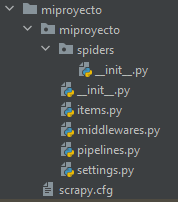
\includegraphics[width=0.3\textwidth]{fig/estructura_proyecto_scrapy.png}
	\caption[Estructura del proyecto recién creado]{Estructura del proyecto recién creado}
	\label{fig:ej11}
\end{figure}

Primero entraremos en el directorio recientemente creado y luego ejecuteremos el comando encargado de crear la Spider.

\begin{verbatim}
	cd miproyecto
	scrapy genspider mispider webausar.com
\end{verbatim}

En caso de no especificar el protocolo usado por la web Scrapy asumirá que usa HTTPS.
\newline
Tras ejecutar el comando la Spider habrá sido generada dentro de la carpeta spiders.

\begin{figure} [h!]
	\centering
	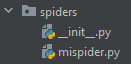
\includegraphics[width=0.3\textwidth]{fig/primera_spider.png}
	\caption[Directorio de almacenamiento de las Spider]{Directorio de almacenamiento de las Spider}
	\label{fig:ej12}
\end{figure}

Una vez abierto el archivo vemos que dispone del siguiente código.

\begin{lstlisting}[language=Python]
	import scrapy
	
	
	class MispiderSpider(scrapy.Spider):
		name = "mispider"
		allowed_domains = ["webausar.com"]
		start_urls = ["https://webausar.com"]
	
	def parse(self, response):
		pass
\end{lstlisting}

Como podemos ver Scrapy usa una programación orientada a objetos, siendo cada Spider una clase representada dentro del proyecto.\newline
Analizando las variables definidas vemos las siguientes, name, nombre por el que debemos referenciar la Spider a la hora de ejecutarla; allowed\_domains, indica que dominios podemos visitar, negando la entrada a cualquier dominio que no este definido en ella, es importante no especificar protocolo, de esta manera funcionara para cualquier web ya sea HTTP como HTTPS que pertenezca a ese dominio, de lo contrario se limitara al protocolo indicado; start\_urls, URL inicial sobre la que se hará la request de petición de datos.\newline
El método parse es aquel al que se envía la respuesta obtenida de la web, para realizar el filtrado de la información, quedándote unicamente con la deseada. Este método es invocado automáticamente por la Spider, sin necesidad real de hacerlo tu manualmente.

\subsection{Proceso de obtención de datos}
Para poder realizar es la extracción de los datos, primero debemos ir a la web deseada e inspeccionar su estructuración. Para ello como ejemplo vamos a usar la web de aemet.\newline

\begin{figure} [H]
	\centering
	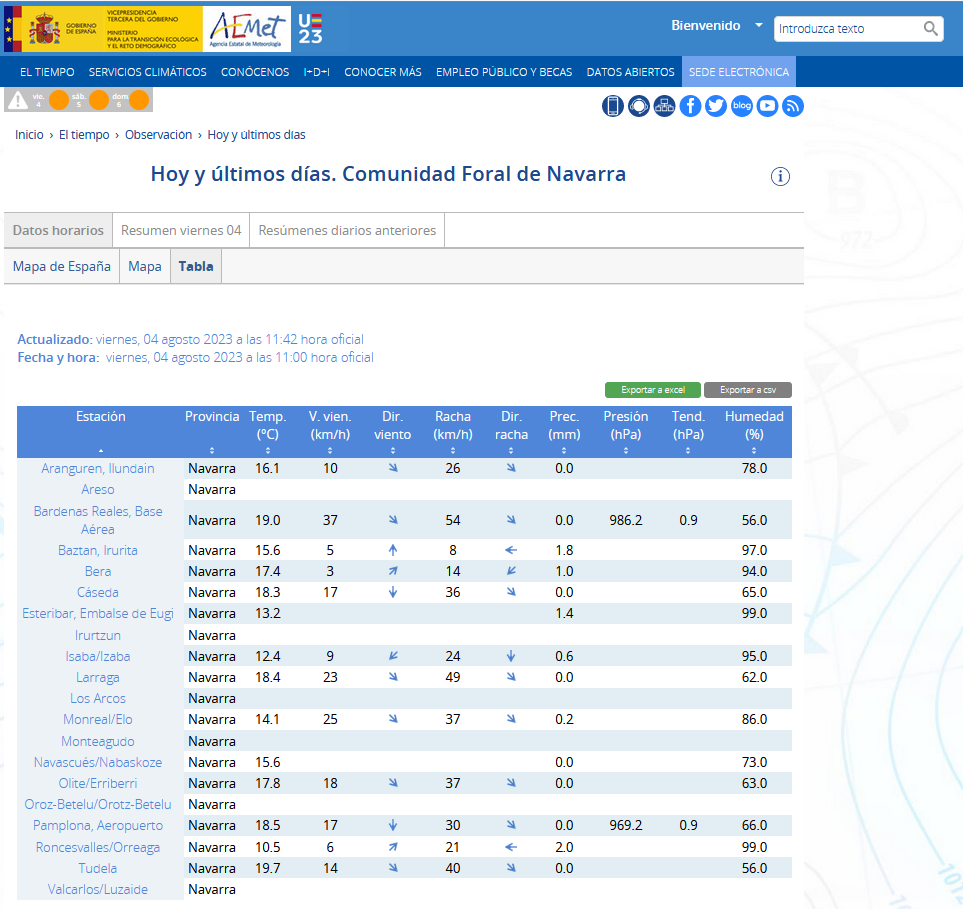
\includegraphics[width=0.8\textwidth]{fig/code_aemet.png}
	\caption[URL de inicio para obtener los códigos de las estaciones de Aemet]{Web de Aemet para obtención de datos}
	\label{fig:ej13}
\end{figure}

Una vez encontrada la web deseada, accediendo mediante el F12 a la herramienta de inspección, buscamos el elemento representativo del dato deseado. En nuestro caso queremos obtener tanto el nombre como el código de la estación. Ambos se encuentran en el mismo elemento que forma la primera columna de la tabla.\newline

\begin{figure} [H]
	\centering
	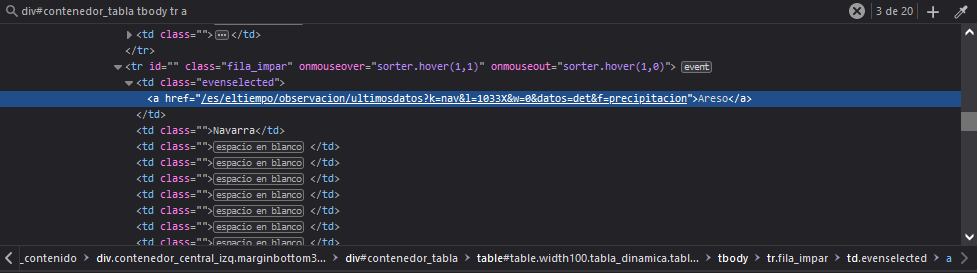
\includegraphics[width=0.9\textwidth]{fig/inspector.png}
	\caption[Inspector de webs de Chrome]{Inspector de webs}
	\label{fig:ej14}
\end{figure}

Como en este caso es posible filtrar fácilmente los datos, los obtendremos todos directamente, aunque lo más común sería obtener las filas primero para luego iterar por cada una de ellas. Para obtenerlos podemos hacerlo mediante el selector de XPath como con el de CSS.\newline

\begin{verbatim}
	rows = response.xpath('//div[@id="contenedor_tabla"]/table/tbody/tr/td/a')
	ó
	rows = response.css("div#contenedor_tabla tbody tr a")
\end{verbatim}

Esto nos devuelve una lista de objetos tipo Selector, cosa que nos permite conforme vamos iterando por cada elemento volver a usar un selector para filtrar unicamente los datos deseados. En nuestro caso.

\begin{verbatim}
	path = rows[i].xpath("@href").get()
	name = rows[i].xpath("./text()").get()
	ó
	path = rows[i].css("*::attr(href)").get()
	name = rows[i].css("*::text").get()
\end{verbatim}

De esta forma, mediante el uso de la función get(), pasamos de tener un objeto Selector a un String. El uso de get() sobre una lista devuelve el primer elemento, en caso de querer transformar toda la lista el método a usar es getall().\newline
\newline
Finalmente, como de la URL obtenida,
\begin{verbatim}
	'/es/eltiempo/observacion/ultimosdatos?k=nav&l=9263X&w=0&datos=det&f=precipitacion'
\end{verbatim}
solo nos interesa el código de la estación (parámetro l de la query), lo filtraremos.
\begin{verbatim}
	code = path.split('&')[1].split('=')[1]
\end{verbatim}

\subsection{Guardado de datos}
Scrapy almacena todos los datos en forma de múltiples diccionarios, tantos como webs usadas. Para acceder a esta información Scrapy nos proporciona dos alternativas, el uso de Items junto a ItemLoaders, siendo clases especificas de Scrapy o, mediante la palabra reservada yield de Python, siendo esta la opción elegida debido a su fácil implementación.
De esta forma escribiremos.
\begin{verbatim}
	yield {
		'estacion': name,
		'codigo': path.split('&')[1].split('=')[1],
	}
\end{verbatim}
Actualmente si se ejecuta la Spider nos imprimiría los datos obtenidos por pantalla, aunque pueden ser almacenados en un fichero tanto CSV como JSON, a la hora de ejecutar la Spider añadiendo en el comando "-o nombre.csv ó -o nombre.json".\newline
Para un uso ligero de forma manual esa alternativa es más que suficiente, pero en nuestro caso, al querer ejecutarlas de forma automática mediante el uso de Runners, debemos implementar una variable llamada custom\_settings para cada una de las Spider. Esta permite, sin la necesidad de modificar el archivo settings.py, añadir configuraciones o dependencias independientes en las Spiders.
\begin{lstlisting}[language=Python]
	custom_settings = {
		'FEEDS': {
			'JSONs/RawCode/codigos_aemet.json': {
				'format': 'json',
				'encoding': 'utf-8',
				'overwrite': True,
			}
		}
	}
\end{lstlisting}
Con esto indicamos que, en la ruta especificada, nos almacene un fichero JSON utf-8 y, que cada vez que se llame a esta Spider sobre-escriba el fichero anterior.

\subsection{Spider básica}
Una vez obtenemos los datos y los podemos almacenar, ya estaria nuestra Spider básica terminada.
\begin{lstlisting}
	import scrapy
	
	
	class AemetCodeSpider(scrapy.Spider):
		name = "aemet_code"
		allowed_domains = ["www.aemet.es"]
		start_urls = ["https://www.aemet.es/es/eltiempo/observacion/"
		"ultimosdatos?k=nav&w=0&datos=det&x=h24&f=precipitacion"]
		custom_settings = {
			'FEEDS': {
				'JSONs/RawCode/codigos_aemet.json': {
					'format': 'json',
					'encoding': 'utf-8',
					'overwrite': True,
				}
			}
		}
	
	def parse(self, response):
		rows = response.css("div#contenedor_tabla tbody tr a")
		
		for row in rows:
		path = row.xpath("@href").get()
		name = row.xpath("./text()").get()
		code = path.split('&')[1].split('=')[1]
		
		yield {
			'estacion': name,
			'codigo': code,
		}
\end{lstlisting}

\chapter[Conclusiones y Trabajo Futuro]{Conclusiones y Trabajo Futuro}
\label{Chap6}

El proyecto a sido llevado a cabo finalmente con las siguientes herramientas, PostGreSQL en la base de datos, Django para la API, Scrapy y Selenium en la plataforma de adquisición de datos y Cron para la automatización de las tareas. Con esto, se ha podido realizar una plataforma, que ejecuta scripts de forma regular en intervalos de tiempo predefinidos para cada página usada, con el fin de no generar más trafico web del realmente necesario.\newline
\newline
En este proyecto se ha creado una arquitectura lo más modular posible, ya sea por el uso de múltiples máquinas virtuales, como por el uso de un entorno virtual por cada uno de los distintos apartados que la forman e, incluso en la forma de codificarla. Lo más intuitiva posible a la hora de poder realizar cambios sobre esta, diferenciando claramente cada elemento.\newline
\newline
El mayor inconveniente en la plataforma creada, es la redundancia de código, al ser múltiples entornos independientes es necesario que gran parte del código se repita en cada uno de ellos. En caso de optar por un único entorno en el que se ejecutara todo, con una clase sobre la que heredar y o una interfaz, sería mucho el código que nos ahorraríamos. Se perdería gran parte de la flexibilidad proporcionada.\newline
\newline
Los entornos virtuales proporcionan un espacio aislado y autónomo en el que trabajar, evitando conflictos entre las dependencias del software. Gracias a esta encapsulación, se pueden instalar bibliotecas, dependencias y herramientas específicas del proyecto, sin afectar el entorno global del sistema. De esta forma, se facilita la creación de grandes aplicaciones, manteniendo cada componente del proyecto en su propio entorno virtual, minimizando los problemas de compatibilidad causados por las dependencias que puedan necesitar.\newline
\newline
Django no cabe duda que es un Framework completo sobre el que trabajar, pero a proporcionado ciertos inconvenientes. Su sistema de gestión de versiones sobre los cambios realizados en la base de datos, supuso tener que rediseñar la arquitectura a una versión más compleja. A su vez, al crear las tablas de la base de datos a partir de los modelos de Django, hizo que no se pudiera hacer uso de una clave primaria compuesta, ya que Django no da soporte a tablas así, siendo una de las peticiones que más ha realizado la comunidad de Django.\newline
\newline
A nivel de obtención de datos, se han presentado múltiples problemas sobre las distintas webs. Como se ha visto en la Sección 2 \ref{Chap2}, algunas no hacen un uso correcto de HTML, creando tablas a partir de CSS sobre elementos \textit{div} en vez de usar las tablas definidas en HTML; o no hacen un buen uso de los atributos \textit{id} y \textit{class}, haciendo la obtención de datos algo tedioso, llegando a tener que filtrar datos mediante los atributos CSS, siendo un claro ejemplo la plataforma de El Agua en Navarra, donde para obtener los códigos de la estación, son filtrados aquellos elementos con el atributo CSS \textit{shape=''rect``}.\newline
\newline
Otros problemas encontrados están relacionados con las coordenadas, pues la web de CHCántabrico no disponge de las coordenadas de las estaciones presentes, siendo un dato que debería ser de acceso público, haciendo que no pueda ser usada sin las coordenadas proporcionadas en una segunda página. Y eso que no se ha llegado a disponer de todas las coordenadas. El segundo problema radica en que todas las estaciones hacen uso de un estándar distinto a la hora de mostrar las coordenadas, por lo que habría que crear un Script capaz de convertir las coordenadas a un mismo estándar para poder ser usadas correctamente.\newline
\newline
Centrado en técnicas de scraping web, este proyecto esta limitado por los datos ofrecidos de forma abierta en la web, siendo su punto débil, aquel del cual no disponemos control alguno. A día de hoy, la plataforma dispone de cuatro fuentes distintas de las cuales obtener datos, pero esta comprometida a que se mantengan invariables en el tiempo. Es por esto, que en un proyecto así necesariamente se debe valorar la búsqueda de datos de forma activa. No solo para su mantenimiento a largo plazo, sino como forma de extender su alcance.\newline
\newline
\backmatter

%%%%%%%%%%%%%%%%%%
%% Bibliography %%
%%%%%%%%%%%%%%%%%%
\input{bibliography/Bibliography.tex}

%%%%%%%%%%%%%%%%%%
%% Word index   %%
%%%%%%%%%%%%%%%%%%
\pagebreak
\cleardoublepage
\phantomsection \label{Index}
\markboth{\glosario}{\glosario}
\addcontentsline{toc}{chapter}{\glosario}
\renewcommand{\indexname}{\glosario}
\printindex
\vfill

%%%%%%%%%%%%%%%%%
%% Anexos	   $$
%%%%%%%%%%%%%%%%%
\pagebreak
\cleardoublepage
\appendix
\markboth{\seccionanexo}{\seccionanexo}
\addcontentsline{toc}{chapter}{\seccionanexo}
\chapter*{\seccionanexo}
\label{anexo}
%%%%%%%%%%%%%%%%%%%%%%%%%%%%%%%%%%%%%%%%%%%%%
%%
%%%%%%%%%%%%%%%%%%%%%%%%%%%%%%%%%%%%%%%%%%%%%


\end{document} 